\documentclass[10pt]{beamer}

% Configuration {{{
\usepackage[utf8]{inputenc}
\usepackage[T2A]{fontenc} % T1 for English
\usepackage[english, russian]{babel}

\usepackage{mathtools}
\usepackage{graphicx}
\usepackage{tikz}
\usepackage[multidot]{grffile}
\usepackage[labelsep=period]{caption}
\usepackage{multirow}

\setbeamertemplate{caption}[numbered]
\setbeamertemplate{navigation symbols}{}
\usefonttheme[onlymath]{serif}
\usepackage{DejaVuSansCondensed} % helvet for English
\usetheme{Madrid}

\linespread{1.2}
% }}}

% Definitions {{{
\def\Lc{{\Lambda_c^+}}
\def\Lcstar{{\Lambda_c^{*+}}{}}
\def\Lca{{\Lambda_c(2765)^+}}
\def\Lcb{{\Lambda_c(2940)^+}}
\def\LcII{{\Lambda_c(2625)^+}}
\def\LcIII{{\Lambda_c(2880)^+}}
\def\LcIIIother{{\Lambda_c(2765)^+}}
\def\ScI{{\Sigma_c(2455)}}
\def\ScIpp{{\Sigma_c(2455)^{++}}{}}
\def\ScIp{{\Sigma_c(2455)^{+}}{}}
\def\ScIz{{\Sigma_c(2455)^{0}}{}}
\def\ScII{{\Sigma_c(2520)}}
\def\ScIIpp{{\Sigma_c(2520)^{++}}{}}
\def\ScIIp{{\Sigma_c(2520)^{+}}{}}
\def\ScIIz{{\Sigma_c(2520)^{0}}{}}
\def\pip{{\pi^+}}
\def\pim{{\pi^-}}
\def\piz{{\pi^0}}
\def\Km{{K^-}}
\def\p{{p}}
\def\Dz{{D^0}}
\def\Dp{{D^+}}
\def\gevcc{{GeV$/c^2$}}
%}}}

% Title and other {{{
\title[Measurements of $\Lambda_c(2880)^+$ in $ee$ annihilation]{
  First observation and measurements of $\Lca$, $\LcIII$, $\Lcb$
  and studies of $\LcIII$ spin-parity -- contents analysis
}
\author[Kerim Guseynov]{
  Kerim Guseynov
  \\[2ex] Based on
  \parbox[t]{20ex}{
    \texttt{arXiv:hep-ex/0010080},
    \texttt{arXiv:hep-ex/0603052},
    \texttt{arXiv:hep-ex/0608043}.
  }
}
\institute[MSU]{Faculty of Physics \\ Moscow State University}
\date{Dec 16, 2022}
%}}}

\begin{document}

\frame[plain]{\titlepage}

\begin{frame}[label=introduction]%{{{
  \frametitle{Introduction}
  \large
  Checks for theoretical predictions:
  \begin{itemize}
    \item Decay channels,
    \item Masses and widths of resonances,
    \item Quantum numbers (spin-parity).
  \end{itemize}
  This information is very useful for construction and tuning of 
  phenomenological models. It may also reveal more CP asymmetry cases.
\end{frame}%}}}

\begin{frame}[label=cleo-det]%{{{
  \frametitle{CLEO detector}
  \centering

  Located at Cornell Electron Storage Ring (Cornell Univ., USA)
  %\\[2ex]
  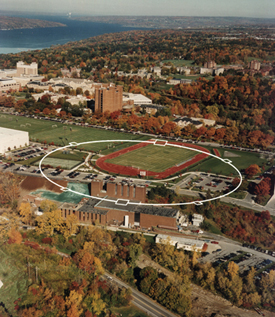
\includegraphics[width=.32\linewidth]{figures/004/cleo-cesr-photo}
  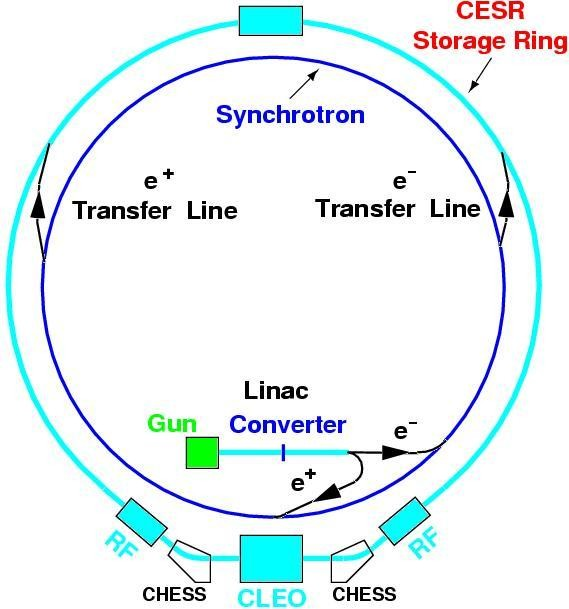
\includegraphics[width=.32\linewidth]{figures/004/cleo-cesr-scheme}
  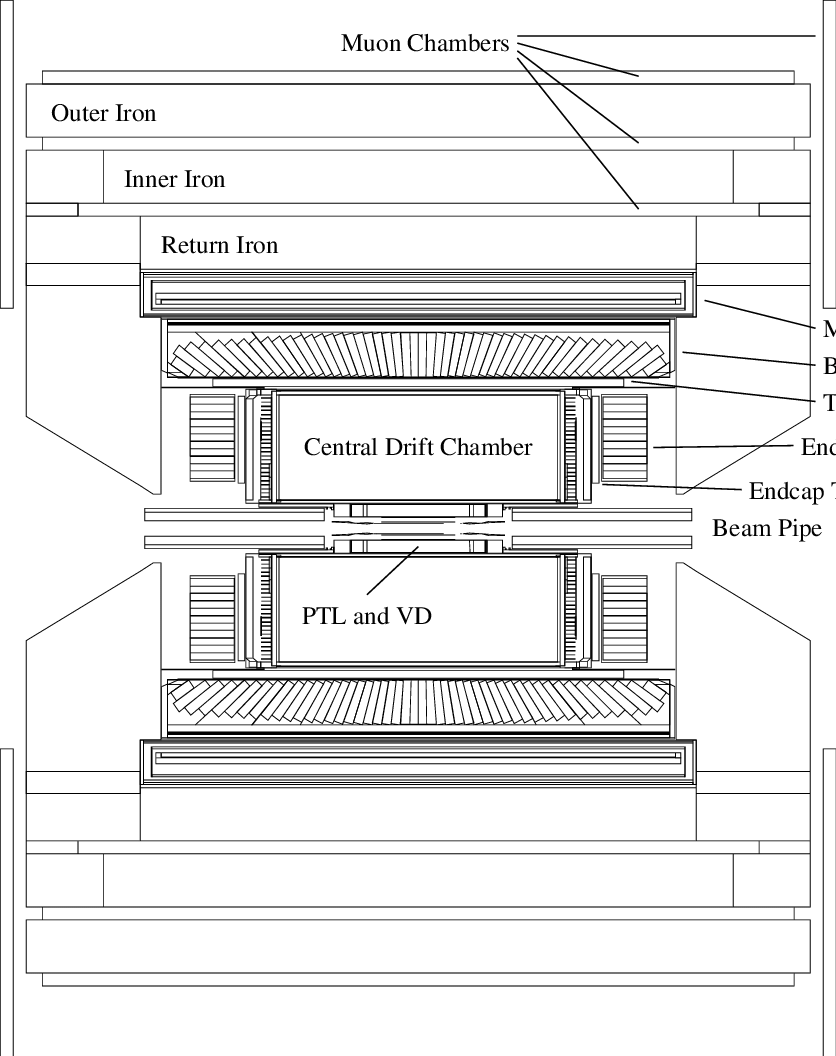
\includegraphics[width=.32\linewidth]{figures/004/cleo-detector}
  \parbox{.32\linewidth}{\centering Real photo}
  \parbox{.32\linewidth}{\centering Scheme}
  \parbox{.32\linewidth}{\centering Detector}
  \\[2ex]
  $ee$ annihilation at $\Upsilon(4S)$
  \\[2ex]
  \parbox{.32\linewidth}{\centering Drift chamber}
  \parbox{.32\linewidth}{\centering EM calorimeter}
  \parbox{.32\linewidth}{\centering Time-of-flight}
\end{frame}%}}}

\begin{frame}[label=cleo-data]%{{{
  \frametitle{Data selection (CLEO)}
  \large

  \begin{itemize}
    \item $\Lc$ reconstructed in 15 modes: combinations of
      $p$, $K$, $\pi$, $\Lambda$, $\Xi$, $\Sigma$, $\phi$.
      Mass requirement: within $1.6\sigma$ of $m(\Lc)_\text{table}$.
    \item Background suppression: cuts on $x_p = p / p_\mathrm{max}$.
      \\ $p_\mathrm{max}$ is the max. the momentum can be given 
      beam energy.
    \item $x_p > 0.5$ rules out the largest comb. bkg. from $B$-mesons.
      \\ Applied to $\Lc$ candidates.
    \item $\Lc$ then combined with two pions:
      $\Lc\pip\pim$.
    \item Further requirement $x_p > 0.7$ for $\Lc\pip\pim$ suggested by 
      kinematics and existing results.
  \end{itemize}
\end{frame}%}}}

\begin{frame}[label=cleo-lcpipi]%{{{
  \frametitle{$\Delta M (\pi\pi) = M(\Lc\pi\pi) - M(\Lc)$ fit}
  \centering
  \parbox{.6\linewidth}{
    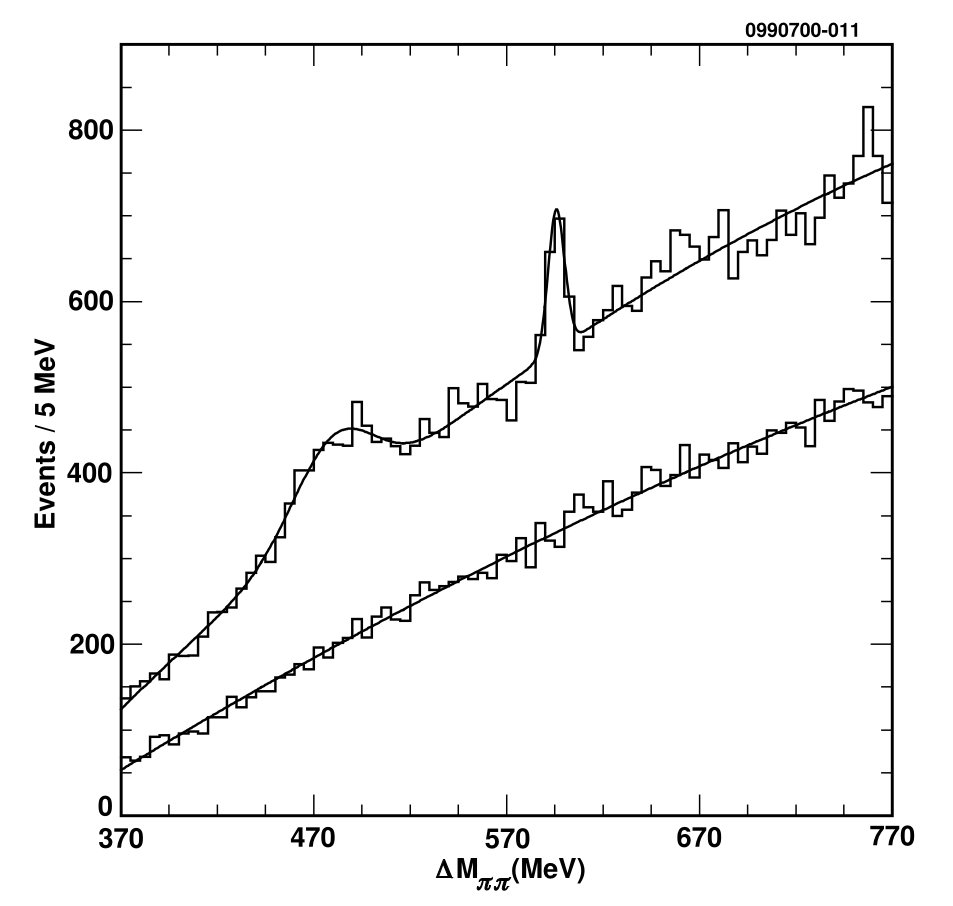
\includegraphics[height=.8\textheight]{figures/004/cleo-fig001}
  } \parbox{.38\linewidth}{
      Lower \\
      \phantom{text} $\Delta M_{\pi\pi} = 480 \pm 3$ MeV \\
      \phantom{text} $\sigma = 21 \pm 3$ MeV \\
      or \\
      \phantom{text} $\Gamma \approx 50$ MeV \\
      \vskip 2ex
      Upper \\
      \phantom{text} $\Delta M_{\pi\pi} = 595.8 \pm 0.8$ MeV \\
      \phantom{text $\Delta M_{\pi\pi} = 595.8$}\! $\pm 2$ MeV \\
      \phantom{text} $\sigma = 4.2 \pm 0.7$ MeV \\
      or \\
      \phantom{text} $\Gamma = 4 \pm 2 \pm 2$ MeV \\
  }
  \small
  Syst. dominated by resolution for $\Gamma$, momentum measurement and fitting for mass.
\end{frame}%}}}

\begin{frame}[label=cleo-lcpi]%{{{
  \frametitle{$\Delta M(\pi) = M(\Lc\pi) - M(\Lc)$ spectrum}
  \centering
  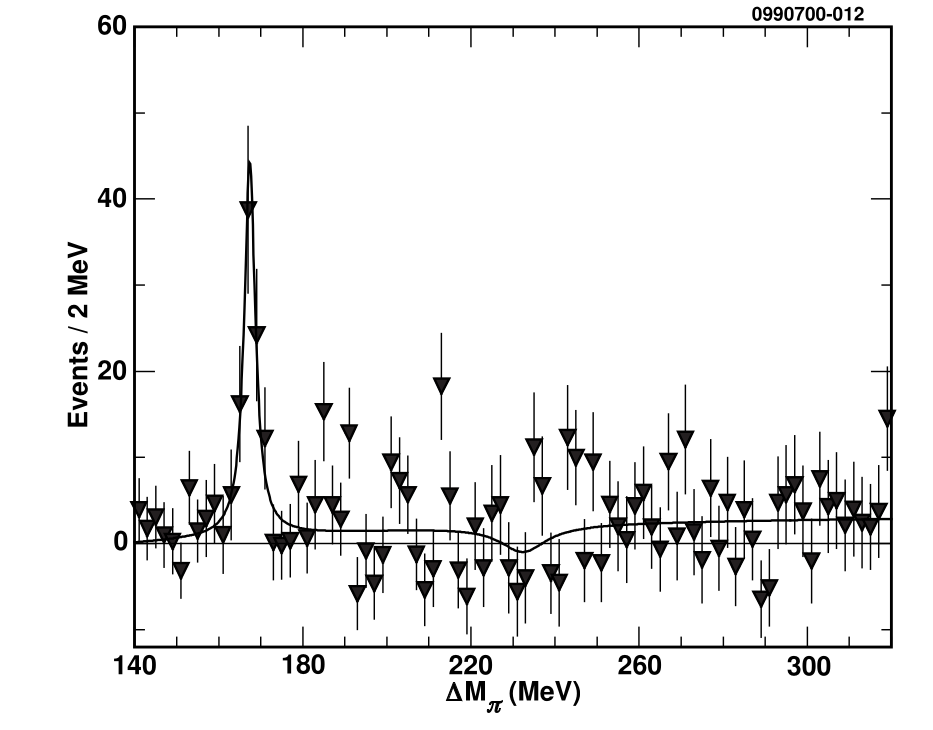
\includegraphics[height=.8\textheight]{figures/004/cleo-fig002}
\end{frame}%}}}

\begin{frame}[label=cleo-lcpipi-from-lcpi]%{{{
  \frametitle{$\Delta M(\pi\pi)$ spectrum from parts of $\Delta M(\pi)$}
  \centering
  \parbox{.6\linewidth}{
    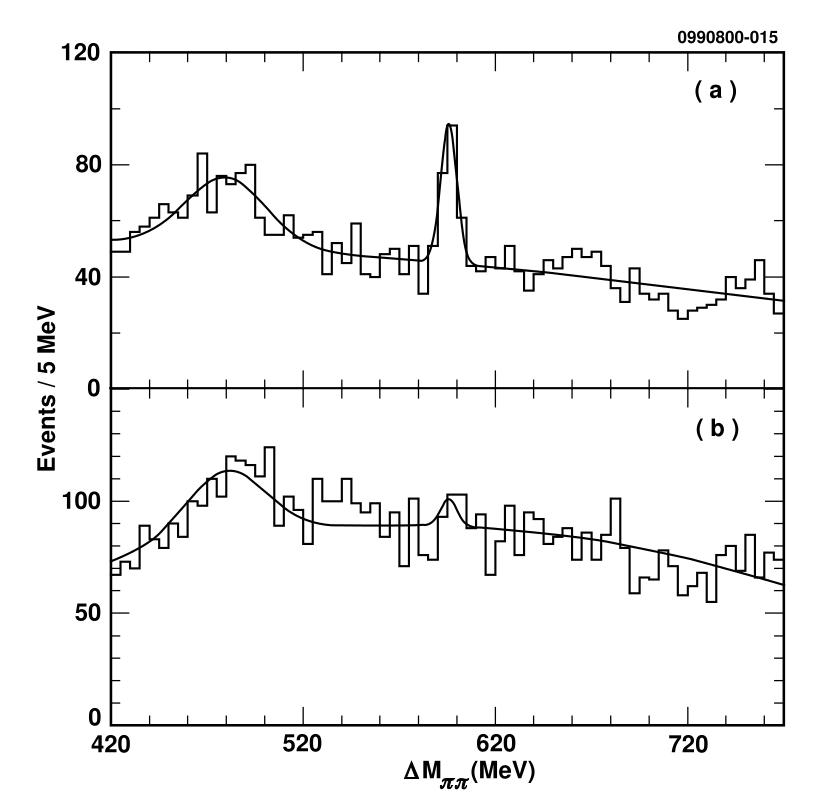
\includegraphics[height=.8\textheight]{figures/004/cleo-fig003}
  } \parbox{.1\linewidth}{
    $\ScI$
    \vskip 4ex
    $\ScII$
  }
\end{frame}%}}}

\begin{frame}[label=cleo-interpretation]%{{{
  \frametitle{Quark states of observed resonances}
  \large
  \begin{itemize}
    \item $\LcIII$ decays into $\ScI\pi$ and $\Lc\pip\pim$ directly.
    \item $\Lca$ possibly decays via all three modes
      $\ScI\pi$, $\ScII\pi$, $\Lc\pip\pim$.
    \item Based on HQET and conservation of both
      $J^P$ and $J^P_\text{diquark}$:
    \item Upper ($\LcIII$):
      \\ $J^P = 1/2^-$, $J^P_\text{diquark} = 0^-$,
      $L = 1$
      \\ or a mixture with $J^P_\text{diquark} = 1^-$,
      $L = 0$
    \item Lower ($\Lca$): very unclear.
      May even be two resonances $30$~MeV apart.
  \end{itemize}
\end{frame}%}}}

\begin{frame}[label=babar-detector]%{{{
  \frametitle{BaBar detector}
  \centering
  Located at PEP-II at SLAC (Stanford University, USA) \\[2ex]
  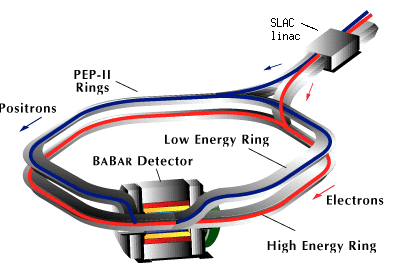
\includegraphics[width=.4\textwidth]{figures/002/babar-scheme}
  \hfill
  
\includegraphics[width=.56\textwidth]{figures/002/upsilon}
  \vskip 3ex
  $ee$ annihilation at $\Upsilon(4S)$ \\[2ex]
  \parbox{.32\linewidth}{\centering Vertex tracker}
  \parbox{.32\linewidth}{\centering Drift chamber}
  \parbox{.32\linewidth}{\centering Cherenkov detector}
\end{frame}%}}}

\begin{frame}[label=babar-data]%{{{
  \frametitle{Data selection (BaBar)}
  \large
  \begin{itemize}
    \item Inclusive $\Dz p$ spectrum investigated.
    \item $\Dz$ reconstructed in $\Km\pip$ and $\Km\pip\pim\pip$
      (fit to a common vertex).
    \item $p$ added using a vertex fit.
    \item Additional requirements:
      \\ $\Delta m = m(\Dz)_\text{reco} - m(\Dz)_\text{table}$,
      \\ $p^*$ -- c.m. momentum of $\Dz p$
         (excludes $B$-meson bkg),
      \\ $\cos\theta$ between $p$ and $ee$ system,
      \\ Based on simulation to maximize significance.
  \end{itemize}
\end{frame}%}}}

\begin{frame}[label=babar-Dp]%{{{
  \frametitle{$\Dz p$ spectrum and fit}
  \centering
  \parbox{.7\linewidth}{
    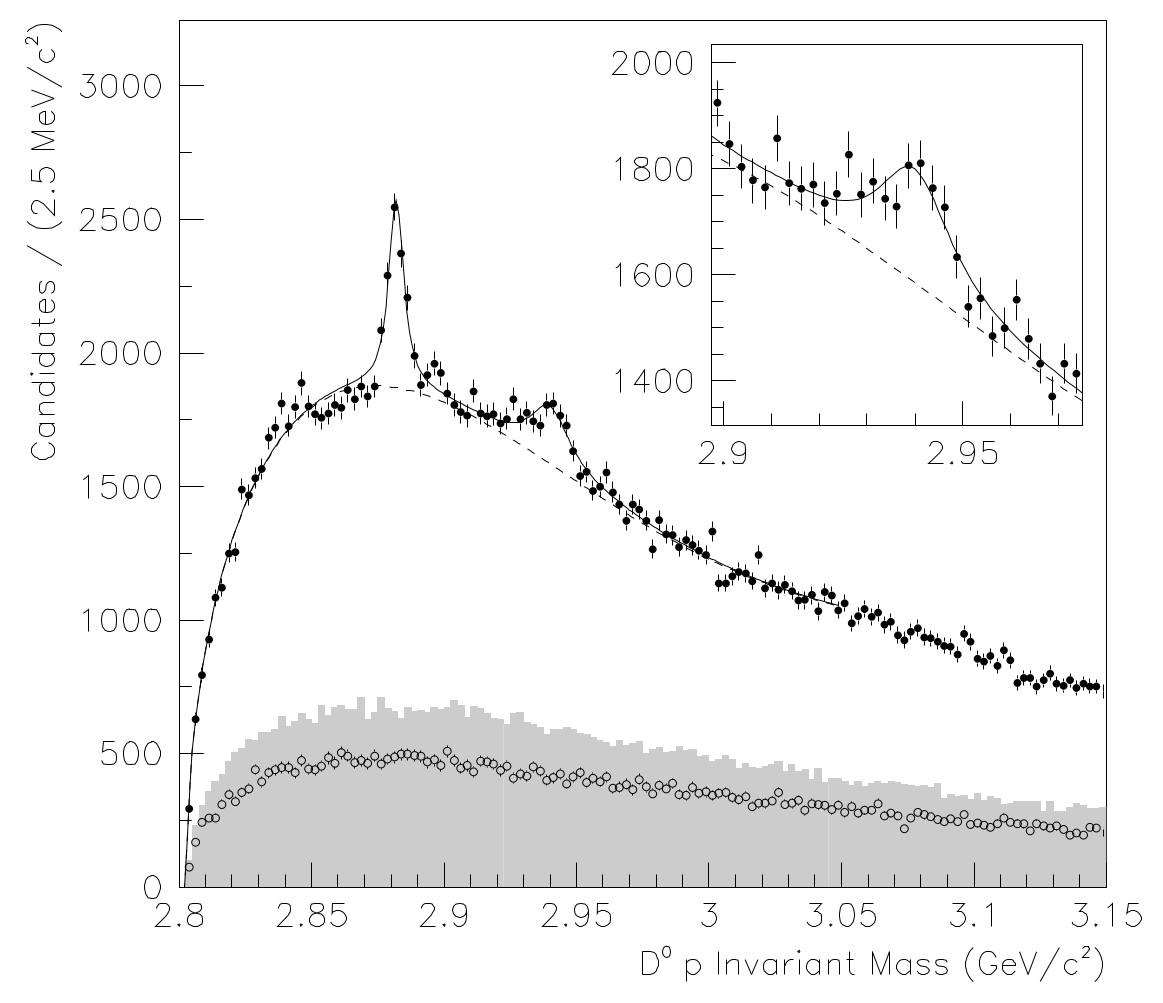
\includegraphics[height=.8\textheight]{figures/004/babar-fig001}
  } \parbox{.28\linewidth}{
    $\Dz$ sidebands in gray,

    $\overline{D}^0$ wrong charge in open circles:

    no structures there.

    \vskip 2ex
    $\LcIII$: \\
    $m = 2881.9 \pm 0.1$ MeV \\
    $\Gamma = 5.8 \pm 1.5$ MeV \\
    \vskip 0ex
    $\Lcb$: \\
    $m = 2939.8 \pm 1.3$ MeV \\
    $\Gamma = 17.5 \pm 5.2$ MeV \\
  }
\end{frame}%}}}

\begin{frame}[label=babar-Dp-alt]%{{{
  \frametitle{$\Dz p$ spectrum: structure at the low end}
  \centering
  \parbox{.52\linewidth}{
    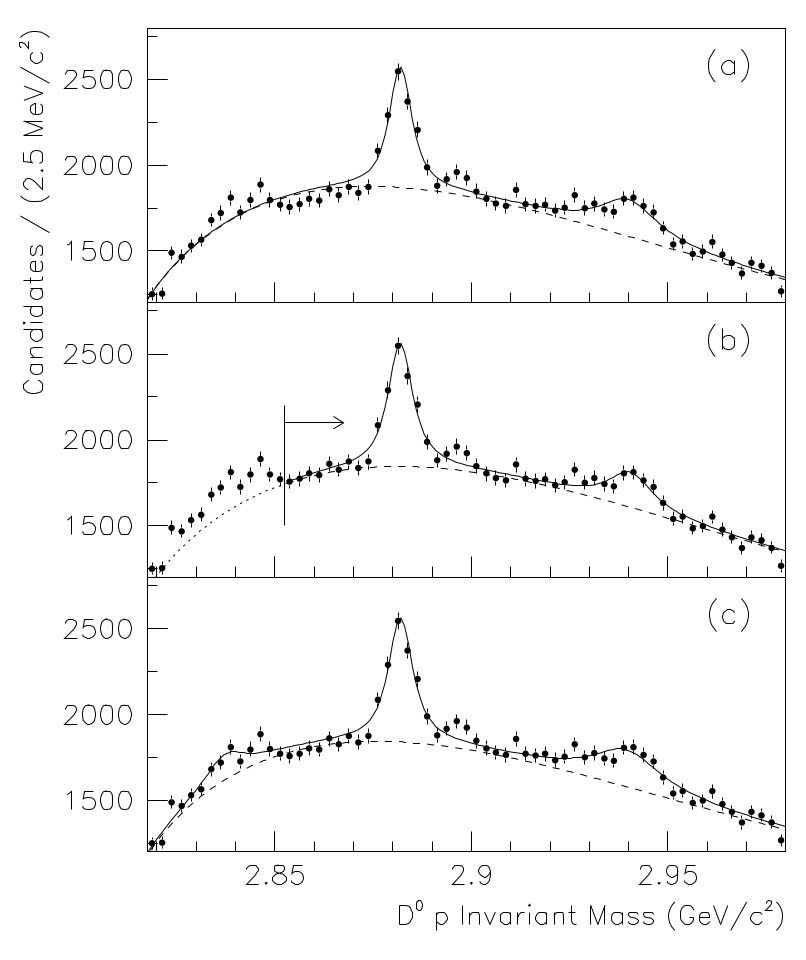
\includegraphics[height=.8\textheight]{figures/004/babar-fig002}
  } \parbox{.28\linewidth}{
    $\Lcb$: \\
    $0.5$ MeV lower mass \\
    $\Gamma = 12.5$ MeV \\

    \flushleft
    Assigned as syst. errors.
  }
\end{frame}%}}}

\begin{frame}[label=babar-results]%{{{
  \frametitle{$\LcIII$ and $\Lcb$ results}
  \large
  \begin{itemize}
    \item Systematics come from fit model
      and the knowledge of $m(\Dz)_\text{table}$.
    \item $\LcIII$:
      $$m = 2881.9 \pm 0.1 \pm 0.5 \text{ MeV}$$
      $$\Gamma = 5.8 \pm 1.5 \pm 1.1 \text{ MeV} $$
    \item $\Lcb$
      $$m = 2939.8 \pm 1.3 \pm 1.0 \text{ MeV} $$
      $$\Gamma = 17.5 \pm 5.2 \pm 5.9 \text{ MeV} $$
    \item $ \dfrac{\sigma\left(\Lcb\right)\,
      \mathcal{B}\left(\Lcb\to\Dz\p\right)}
      {\sigma\left(\LcIII\right)\,
      \mathcal{B}\left(\LcIII\to\Dz\p\right)}
      = 0.81 \pm 0.13 \pm 0.35
      $
  \end{itemize}
\end{frame}%}}}

\begin{frame}[label=babar-tests]%{{{
  \frametitle{Tests for $\Lcb$}
  \centering
  \parbox{.48\linewidth}{
    \begin{itemize}
      \item Not coming from $K$ or $\pi$ misidentified as $p$:
        such spectra exhibit no peaks.
      \item Not coming from a heavier narrow $\Lcstar$
        decaying into $D^* p$:
        no peaks in $D^* p$ spectra.
      \item Not coming from a heavier $\Lcstar$
        decaying into $D^0 \Sigma^+$:
        kinematics of $D^0 \Sigma^+$ are different.
      \item $\Lcb$ is not a $\Sigma_c^{*+}$:
        no doubly-charged state in $\Dp p$.
    \end{itemize}
  } \parbox{.5\linewidth}{
    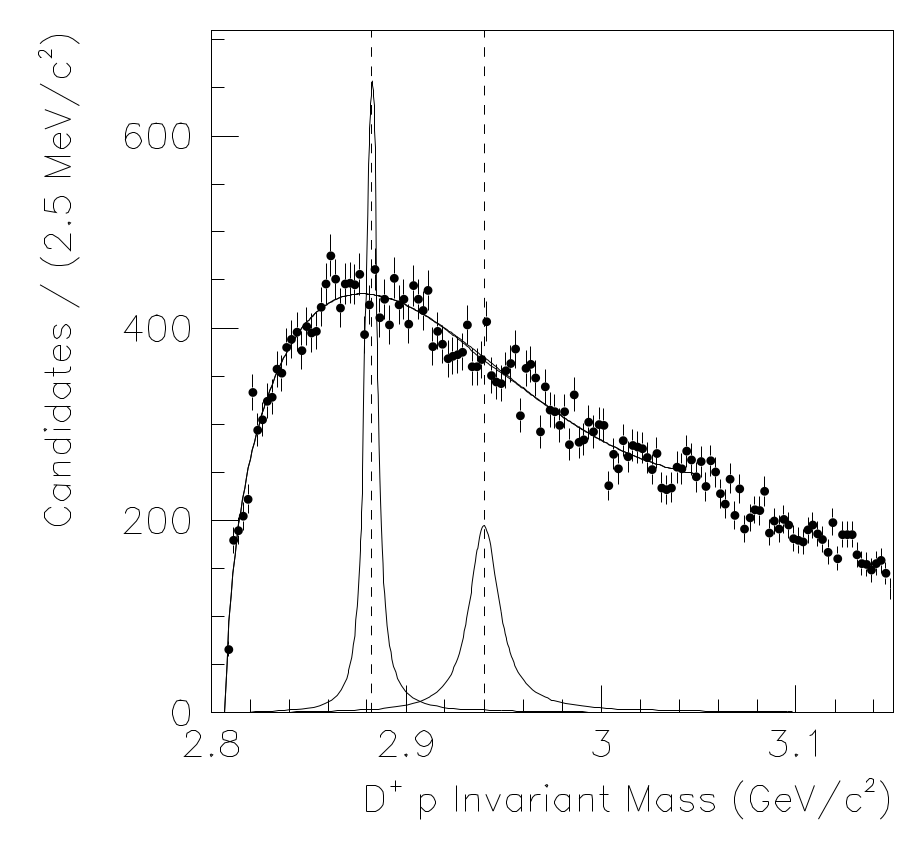
\includegraphics[width=\linewidth]{figures/004/babar-fig003}
  }
\end{frame}%}}}

\begin{frame}[label=babar-conclusion]%{{{
  \frametitle{Conclusions about $\LcIII$, $\Lcb$}
  \Large
  \begin{itemize}
    \item First observation of $\Dz p$ decay mode.
      \\ (and, to this day, the only one)
    \item $\Lcb$ not observed in $\Lc\pip\pim$ by CLEO.
      \\ Why is $\Dz p$ favored in spite of phase space?
    \item $\LcIII$ consistent with CLEO measurement.
  \end{itemize}
\end{frame}%}}}

\begin{frame}[label=belle-detector]%{{{
  \frametitle{Belle detector}
  \centering

  {\small Located at KEKB at KEK
  (High Energy Accelerator Research Organization, Japan)}
  \vskip 1ex
  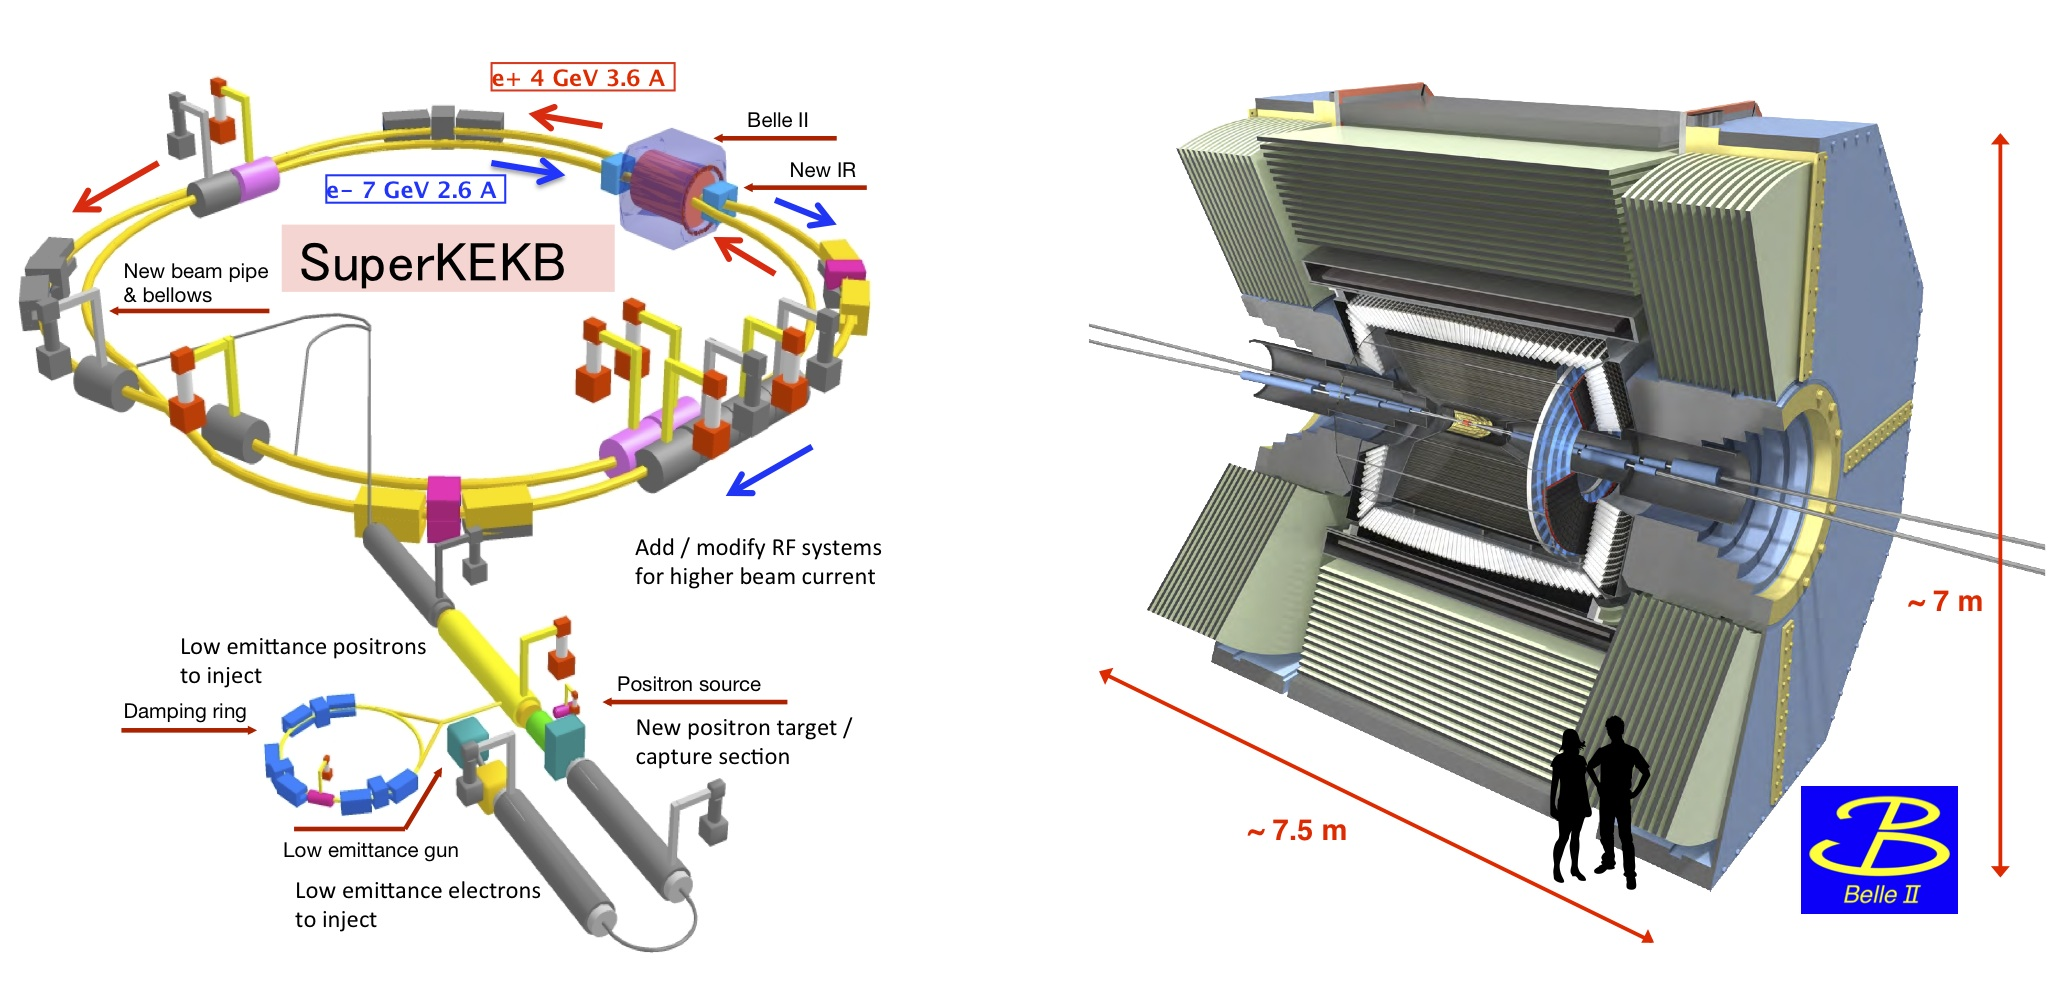
\includegraphics[width=.8\linewidth]{figures/004/belle-ring-detector}
  \vskip 1ex
  $ee$ annihilation at $\Upsilon(4S)$ \\[2ex]
  \parbox{.32\linewidth}{\centering Vertex detector}
  \parbox{.32\linewidth}{\centering Drift chamber}
  \parbox{.32\linewidth}{\centering Cherenkov detector}
  \vskip 1ex
  \parbox{.48\linewidth}{\centering Time-of-flight counters}
  \parbox{.48\linewidth}{\centering Scintillator}
\end{frame}%}}}

\begin{frame}[label=belle-data]%{{{
  \frametitle{Data selection (Belle)}
  \large
  \begin{itemize}
    \item $\Lc$ reconstructed in $\Lc\to\p\Km\pip$.
    \item $\Lc$ mass required to be within $1.6\sigma$
      of existing measurements.
    \item Particle identification applied.
    \item Cut on $x_p > 0.7$ for $\Lc\pip\pim$ candidates.
    \item For mass fits, $\Lc\pi$ mass cut to $\ScI$ region.
      \\ This reduces the signal, but heavily suppresses the bkg.
  \end{itemize}
\end{frame}%}}}

\begin{frame}[label=belle-lcpipi]%{{{
  \frametitle{$\Lc\pip\pim$ spectrum and fit}
  \parbox{.65\linewidth}{
    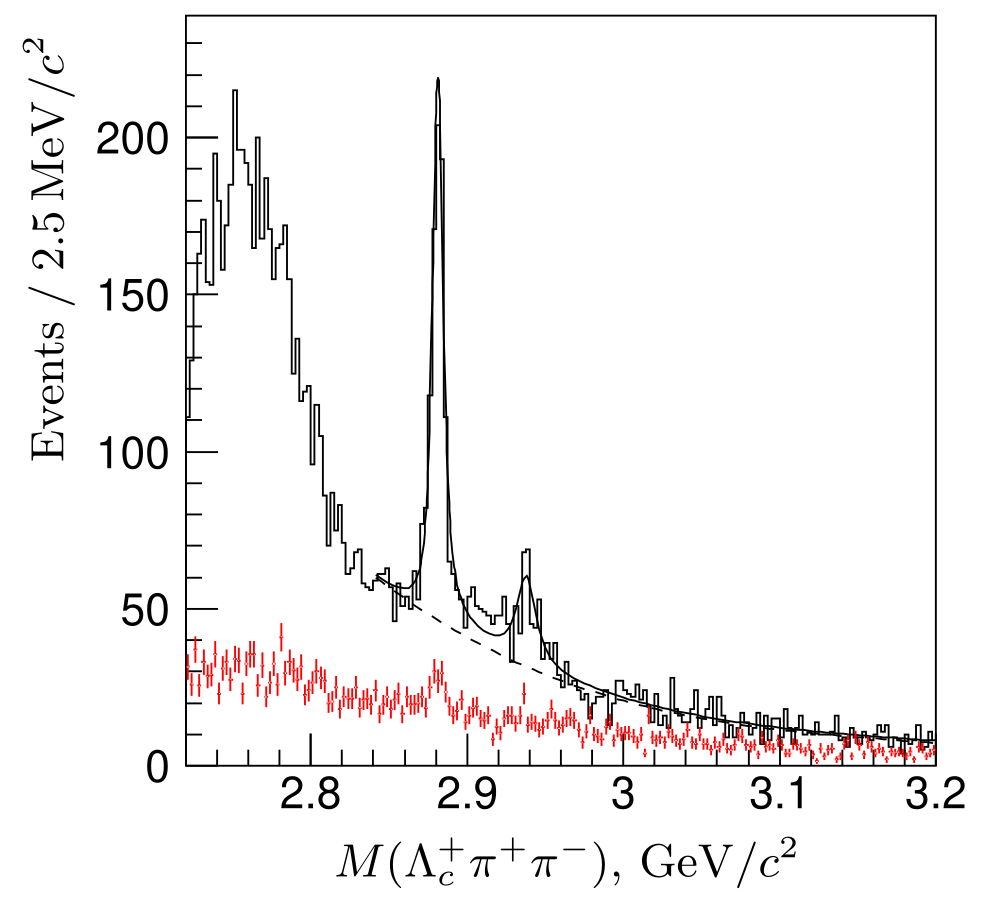
\includegraphics[height=.8\textheight]{figures/004/belle-fig001}
  } \parbox{.34\linewidth}{
    $\LcIII$:
    \\ $m = 2881.2 \pm 0.2 \pm 0.4$ MeV
    \\ $\Gamma = 5.8 \pm 0.7 \pm 1.1$ MeV
    \vskip 2ex
    $\Lcb$:
    \\ $m = 2938.0 \pm 1.3^{+2.0}_{-4.0}$ MeV
    \\ $\Gamma = 13^{+8}_{-5}{}^{+27}_{-7}$ MeV
  }
\end{frame}%}}}

\begin{frame}[label=belle-mass-syst]%{{{
  \frametitle{$\LcIII$ and $\Lcb$ measurements systematics}
  \large
  \begin{itemize}
    \item 4th-order polynomial instead of 3rd.
      \\ Inverse 3rd-order polynomial.
    \item Include $\LcIIIother$ region in the fit: Breit-Wigner.
    \item Selection requirements.
    \item Uncertainty in detector resolution.
    \item Poor fit quality between 2880 and 2940~MeV.
  \end{itemize}
  \vskip 2ex
  Main sources: $\LcIIIother$ and region between 2880 and 2940~MeV.
\end{frame}%}}}

\begin{frame}[label=belle-lcpi-bins]%{{{
  \frametitle{$\LcIII$ yields in $\Lc\pi$ mass bins}
  \centering
  \parbox{.65\linewidth}{
    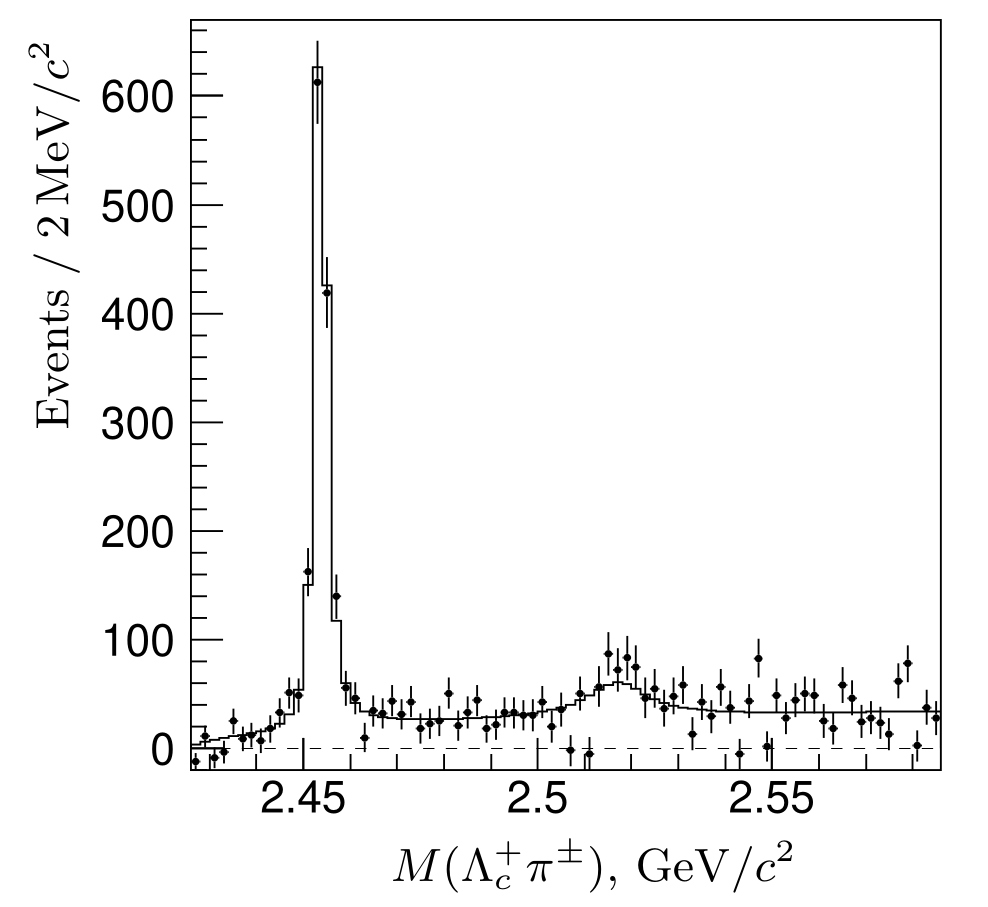
\includegraphics[height=.8\textheight]{figures/004/belle-fig002}
  } \parbox{.34\linewidth}{
    \flushleft
    $\LcIII$ and $\Lcb$ models are fixed in $\Lc\pip\pim$ fits.
    \vskip 1ex
    Non-res. component shape in $\Lc\pi$ is taken from simulation.
    \vskip 3ex
    $\ScI$ parameters floated.
    \vskip 1ex
    $\ScII$ parameters fixed.
  }
\end{frame}%}}}

\begin{frame}[label=belle-br-syst]%{{{
  \frametitle{$\LcIII$ branching ratios systematics}
  \centering
  \vskip -\baselineskip
  $$\dfrac{\Gamma(\ScI\pi)}{\Gamma(\Lc\pip\pim)}
  = 0.404 \pm 0.021 \pm 0.014, \quad
  \dfrac{\Gamma(\ScII\pi)}{\Gamma(\Lc\pip\pim)}
  =0.091 \pm 0.025 \pm 0.010 $$
  $$\dfrac{\Gamma(\ScII\pi)}{\Gamma(\ScI\pi)}
  = 0.225 \pm 0.062 \pm 0.025 $$
  \vfill
  \begin{itemize}
    \item Parameters of $\LcIII$.
    \item $\Lc\pip\pim$ fit interval.
    \item Bkg shape in $\Lc\pip\pim$.
    \item $\ScII$ parameters in $\Lc\pi$ fit.
    \item Non-resonant shape in $\Lc\pi$ fit:
      \\ 2nd-order polynomial with threshold,
      \\ 3rd-order polynomial.
  \end{itemize}
\end{frame}%}}}

\begin{frame}[label=belle-lc2880-spin]%{{{
  \frametitle{$\LcIII\to\Sigma_c\pi$
  yields in $\cos\theta$ and $\cos\phi$ bins}
  \centering
  $\theta$ -- between $\pi$ in $\LcIII$ rest frame and $\LcIII$ boost.
  \vskip .5ex
  $\phi$ -- between $ee\to\LcIII X$ reaction plane
  and plane formed by $\pi$ momentum and $\LcIII$ boost.
  \vskip 1ex
  \parbox{.48\linewidth}{
    \vskip -1ex
    \begin{tikzpicture}[x=.01\linewidth, y=.01\linewidth]
      \path (0, 0) node{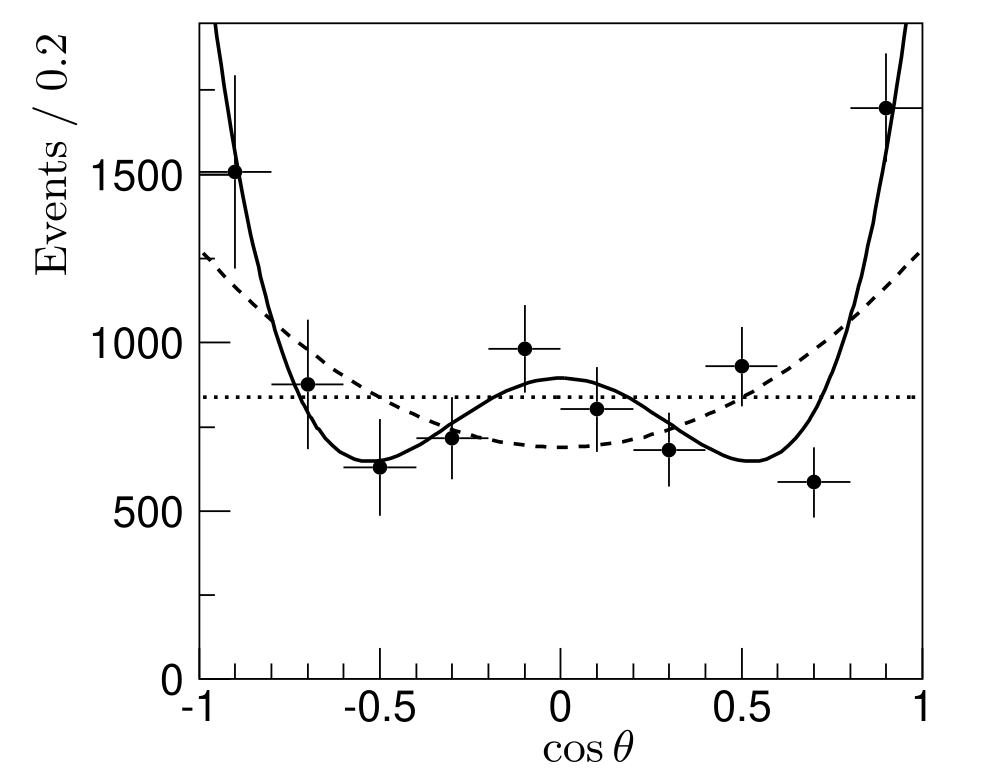
\includegraphics[width=\linewidth]{figures/004/belle-fig003-1}};
      \path (7, 30) node{
        $\frac{1}{2}$ vs $\frac{3}{2}$ vs $\frac{5}{2}$
      };
    \end{tikzpicture}
  }
  \parbox{.48\linewidth}{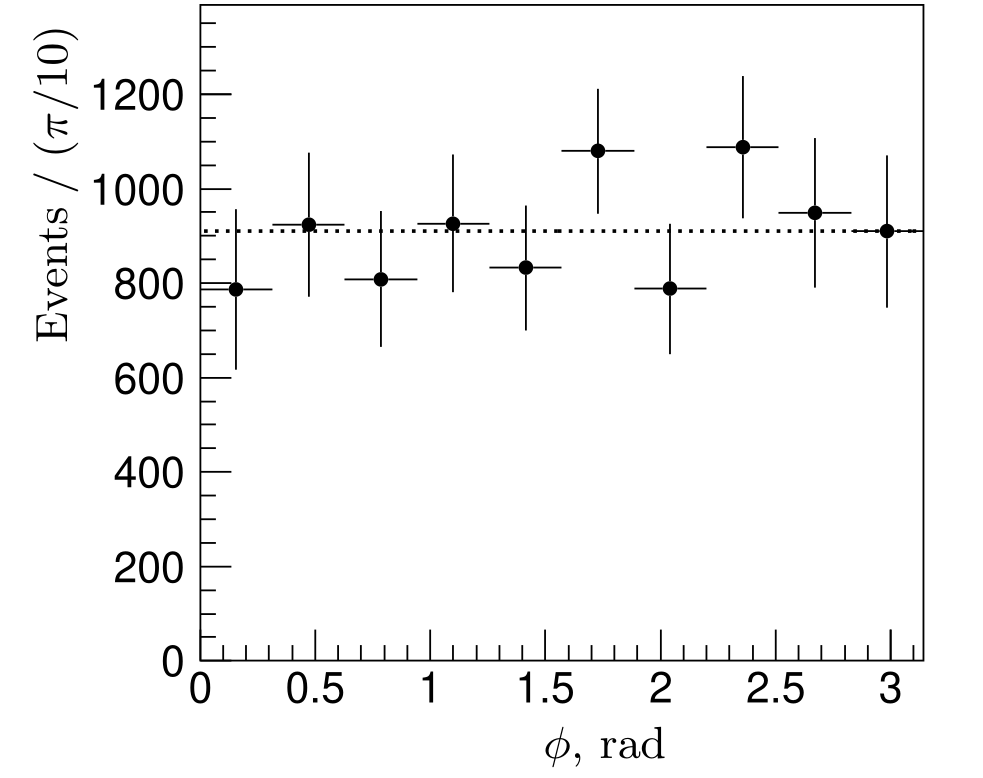
\includegraphics[width=\linewidth]{figures/004/belle-fig003-2}}
  \vskip 1ex
  $\dfrac{\Gamma(\ScII\pi)}{\Gamma(\ScI\pi)} = 1.4$
  for ${5\over2}^-$ and $0.23$--$0.36$ for ${5\over2}^+$.
  Measured $0.225 \pm 0.067$
\end{frame}%}}}

\begin{frame}[label=belle-results]%{{{
  \frametitle{Results of $\LcIII$ spin measurement}
  \large
  \begin{itemize}
    \item Spin $\frac{5}{2}^+$ hypothesis strongly favored.
    \item Spin $\frac{1}{2}^+$ hypothesis exclusion level: 5.5 sigma.
    \item Spin $\frac{3}{2}^+$ hypothesis exclusion level: 4.5 sigma.
    \item Spin-parity $\frac{5}{2}^+$ is favored.
    \item $\LcIII$ belongs to the sequence \\[1ex]
      \hfill
      $\Lc$     $\left(\frac{1}{2}^+\right)$,
      $\LcII$   $\left(\frac{3}{2}^-\right)$,
      $\LcIII$  $\left(\frac{5}{2}^+\right)$.
      \hfill\null
  \end{itemize}
\end{frame}%}}}

\end{document}
